\section{Michalina Kujawa}
\label{sec:mkujawa}

I added a photo of my favourite sport discipline %(see Figure~\ref{fig:horse}).

\begin{figure}[H]
    \centering
    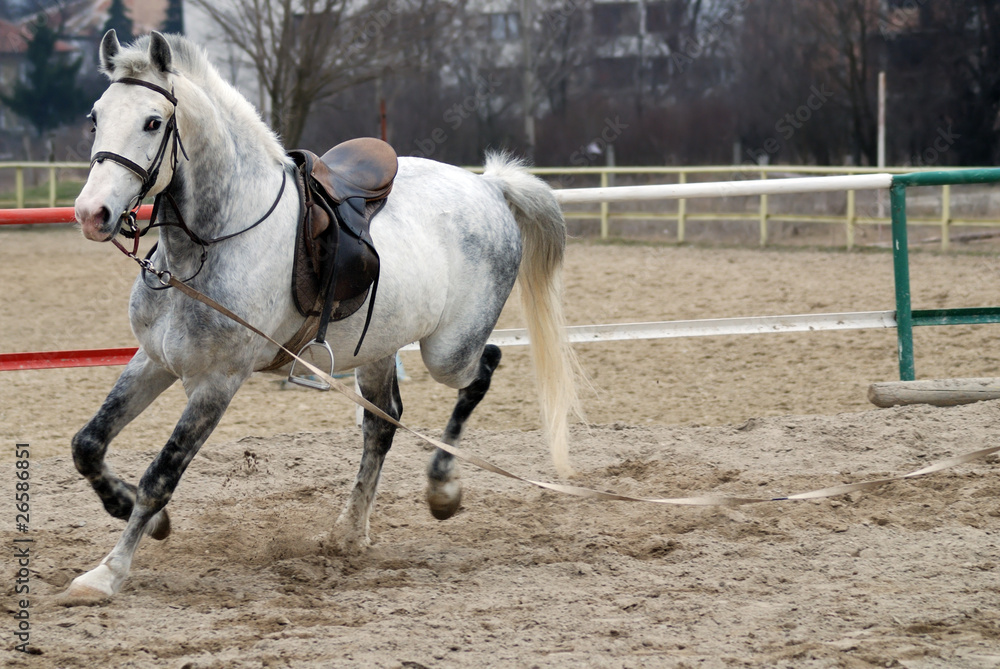
\includegraphics[width=0.7\textwidth]{pictures/pic_MK.jpg} 
    \caption{This horse is wonderful.}
    \label{fig:horse}
\end{figure}

Horse riding, often referred to as equestrianism, is a centuries-old and timeless pursuit that combines athleticism, grace, and a profound connection with one of nature's most magnificent creatures. It is not just a sport but a harmonious partnership between horse and rider, where communication occurs through subtle cues and mutual trust. The rhythmic clip-clop of hooves and the gentle sway of the saddle create a unique sensory experience that transports riders to a world of serenity and freedom. Whether it's a leisurely trail ride through the tranquil countryside or the exhilaration of competing in a thrilling showjumping event, horse riding offers a diverse range of experiences for riders of all levels, from novices to seasoned equestrians.

Beyond the physical and emotional benefits, horse riding fosters a deep appreciation for these majestic animals and the beauty of the natural world. It teaches riders the values of patience, responsibility, and respect for both the horse and the environment. The bond formed between a rider and their horse is one of profound trust and companionship, and it's a connection that transcends language, fostering an unspoken understanding between the two. Whether you ride for recreation or competition, horse riding is a remarkable journey that brings riders closer to nature while unlocking the joy of adventure, teamwork, and personal growth in the process.


%Table~\ref{tab:random_numbers} represents random numbers. 

\begin{table}[H]
    \centering
    \begin{table}[htbp]
\centering
\begin{tabular}{||c c c c c c||} 
 \hline
 Years & Football & Basketball & Volleyball & Swimming & Cycling \\ [0.5ex] 
 \hline\hline
 2000-2005 & 36\% & 47\% & 12\% & 24\% & 30\% \\ 
 \hline
 2006-2011 & 40\% & 38\% & 23\% & 31\% & 27\% \\
 \hline
 2012-2017 & 67\% & 35\% & 49\% & 35\% & 21\% \\
 \hline
 2018-2023 & 65\% & 29\% & 50\% & 55\% & 15\% \\
 \hline
\end{tabular}
\label{tab:random_numbers}
\caption{The most likely chosen sports in recent years.}
\end{table}
\end{table}

Here is also a worth seeing equation: \[P^2=p(p-a)(p-b)(p-c)\]

This formula allows you to calculate the area of a triangle ( p = half of the circumference; a,b,c = sides of the triangle ) 


%\hfill\break 
This is the list of 5 most likely visited countries in recent years:
\begin{itemize}
  \item France
  \item Spain
  \item USA
  \item China
  \item Italy
\end{itemize}

%\hfill\break
This is the list of 5 less likely visited countries in recent years:
\begin{enumerate}
  \item Ukraine
  \item Singapore
  \item Saudi Arabia
  \item Korea
  \item Vietnam
\end{enumerate}